% !TEX root = ../ITGO.tex

\section*{GKLS class of functions}

We used C-ITGO to optimize the 800 functions generated by the GKLS generator \citep{GKLS}, considering the differentiable type (“D”). There are 100 functions for each setup, namely, with 2, 3, 4 and 5 variables, each consisting of an “easy” and “hard” case. The parameters used for each class of functions follows:


% !TEX root = ../main.tex

\begin{table*}[h]
\tiny
\begin{center}
\def\arraystretch{1.5}%
\begin{tabular}{ | P{1.0cm} | P{1.0cm} | P{1.0cm} | P{1.0cm} | P{1.0cm} | P{1.0cm} | }

\cline{2-6}
\multicolumn{1}{c|}{} & \textbf{N} & \textbf{M} & \bm{$\Delta$} & \bm{$r^*$} & \bm{$\rho^*$} \\
\hline

\multirow{ 4}{*}{Easy} & 2 & 10 & 10E-4 & 0.90 & 0.2 \\
& 3 & 10 & 10E-6 & 0.66 & 0.2 \\
& 4 & 10 & 10E-6 & 0.66 & 0.2 \\
& 5 & 10 & 10E-7 & 0.66 & 0.3 \\

\hline

\multirow{ 4}{*}{Hard} &  2 & 10 & 10E-4 & 0.90 & 0.1 \\
& 3 & 10 & 10E-6 & 0.9 & 0.2 \\
& 4 & 10 & 10E-6 & 0.9 & 0.2 \\
& 5 & 10 & 10E-7 & 0.66 & 0.2 \\

\hline



\end{tabular}
\end{center}
\vspace{-0.6cm}
\caption{Parameters used in the GKLS generator.}
\label{tab:MD}
\end{table*}


\noindent
Where:


\begin{itemize}

\item $N$ - problem dimension;
\item $M$ - number of local optima;
\item $\Delta$ - accuracy coefficient;
\item $\rho^*$ - radius of the attraction region of the global optimum;
\item $r^*$ - distance from the global optimum to the vertex of the paraboloid.

\end{itemize}


We compared the results achieved by C-ITGO against a number of deterministic global optimization methods. We used the approach described in \cite{NAT} to compare meta-heuristics with deterministic algorithms. For each of the 100 problems of a given class, we ran C-ITGO 100 times, saving the mean number of function/gradient evaluations for that problem. We stopped when the best solution $\bm{x}'$ found in a run satisfies:\\[-2.5em]

\begin{equation}\label{eq:Convergence}
    |x'(i) - x^*(i)| \leq \sqrt{\Delta}(b(i) - a(i)), \qquad 1 \leq i \leq N,
\end{equation}


\noindent
where $\bm{x}^*$ is the global optimal solution and $\bm{a}$ and $\bm{b}$ are respectively the lower and upper bound vectors defining the problem's domain.

The deterministic methods used for comparison are DIRECT \citep{DIRECT}, DIRECT-L \citep{DIRECTL}, ADC \citep{ADC}, SGEO-QN \citep{SGEO} (using $P_4$) and DIRECT-KS \citep{ADC2}. 

The parameters used in C-ITGO are presented in Table \ref{tab:ITGO}. Because the GKLS classes of problems are unconstrained, the $\alpha$ parameter is omitted and the stochastic topographical heuristic is not used. The L-BFGS algorithm was used as the local search for unconstrained smooth optimization. A very small number of local search calls were necessary to reach convergence.

\documentclass[A4, 11pt, preprint]{elsarticle}

%\usepackage{cite}

\usepackage[fleqn]{amsmath}
\usepackage{amssymb}
\usepackage{algorithm}
\usepackage{algpseudocode}
\usepackage{etoolbox}
\usepackage{setspace}
\usepackage{lineno,hyperref}


\makeatletter
\AfterEndEnvironment{algorithm}{\let\@algcomment\relax}
\AtEndEnvironment{algorithm}{\kern2pt\hrule\relax\vskip3pt\@algcomment}
\let\@algcomment\relax
\newcommand\algcomment[1]{\def\@algcomment{\footnotesize#1}}


\renewcommand\fs@ruled{\def\@fs@cfont{\bfseries}\let\@fs@capt\floatc@ruled
  \def\@fs@pre{\hrule height.8pt depth0pt \kern2pt}%
  \def\@fs@post{}%
  \def\@fs@mid{\kern2pt\hrule\kern2pt}%
  \let\@fs@iftopcapt\iftrue}
\makeatother


\makeatletter
\g@addto@macro{\endtabular}{\rowfont{}}% Clear row font
\makeatother
\newcommand{\rowfonttype}{}% Current row font
\newcommand{\rowfont}[1]{% Set current row font
   \gdef\rowfonttype{#1}#1%
}


\usepackage{array}

\usepackage{booktabs}

\newcolumntype{P}[1]{>{\centering\arraybackslash}p{#1}}

\usepackage{stfloats}

\usepackage{url}

\usepackage{graphicx}

\usepackage{multicol}

\usepackage{caption}
\usepackage{subcaption}

\usepackage{siunitx}

\usepackage[hang,flushmargin]{footmisc}

%\usepackage{auto-pst-pdf}

\usepackage{multirow}
\usepackage{array}
\usepackage{tabu}

\captionsetup{font=footnotesize}


\newcommand{\tcent}[1]{\multicolumn{1}{c|}{#1}}


%%%%%%%%% DRAWING %%%%%%%%%


\usepackage{bera}
\usepackage{pstricks}
\usepackage[T1]{fontenc}
\usepackage{epsfig}
\usepackage{pst-grad} % For gradients
\usepackage{pst-plot} % For axes
\usepackage[space]{grffile} % For spaces in paths
\usepackage{etoolbox} % For spaces in paths
\usepackage{pst-node,pst-blur,pstricks-add}
\usepackage[utf8]{inputenc}

\usepackage{bm}



%%%%%%%%%%%%%%%%%%%%%%%%%%%%%%%%%%%%%%%%




\newcommand{\fnt}[1]{\fontsize{#1}{#1}\selectfont}
\newcommand{\fntt}{\fnt{7}}


\newcommand{\bbfamily}{\fontencoding{U}\fontfamily{bbold}\selectfont}
\DeclareMathAlphabet{\mathbbold}{U}{bbold}{m}{n}

\makeatletter
\renewcommand{\ALG@beginalgorithmic}{\fnt{8}}
\makeatother

\newcommand\numberthis{\addtocounter{equation}{1}\tag{\theequation}}


% correct bad hyphenation here
\hyphenation{op-tical net-works semi-conduc-tor}


\newcolumntype{?}{!{\vrule width 1pt}}



\iffalse

\usepackage{fancyhdr}

\pagestyle{fancy}
\newcommand\shorttitle{{\fontfamily{zlmtt}\selectfont\fnt{9} Improvements on Biased Random-Key Genetic Algorithms \\ for Non-Linearly Constrained Global Optimization}}
\newcommand\authors{{\fontfamily{zlmtt}\selectfont\fnt{9} M. P. Ferreira, M. L. Rocha, A. J. Silva Neto}}
\fancyhf{}
\renewcommand\headrulewidth{0pt}
\fancyhead[C]{%
\ifodd\value{page}
  \small\scshape\authors
\else
  \small\scshape\shorttitle
\fi }

\fancyhead[R]{\thepage\ifodd\value{page}\else\hfill\fi}


\makeatletter
\def\blfootnote{\gdef\@thefnmark{}\@footnotetext}
\makeatother

\fi



\captionsetup[algorithm]{format=hang,singlelinecheck=false}

%\renewcommand{\thesection}{\arabic{section}} 
%\renewcommand{\thesubsection}{\thesection.\arabic{subsection}}




% ALGORITHMS

\usepackage{tikz}


\newcommand\tikzmark[1]{%
  \tikz[remember picture,overlay]\node[inner sep=2pt] (#1) {};}
\newcommand\DrawBox[3][]{%
  \tikz[remember picture,overlay]\draw[#1] ([xshift=-3.5em,yshift=7pt]#2.north west) rectangle (#3.south east);}

\algnewcommand\algorithmicinput{\textbf{Input:}}
\algnewcommand\INPUT{\item[\algorithmicinput]}

\algnewcommand\algorithmicoutput{\textbf{Output:}}
\algnewcommand\OUTPUT{\item[\algorithmicoutput]}

\algnewcommand\algorithmicLet{\textbf{Let:}}
\algnewcommand\LET{\item[\algorithmicLet]}



\usepackage{varwidth}% http://ctan.org/pkg/varwidth

\newcommand\NoThen{\renewcommand\algorithmicthen{}}
\newcommand\ReThen{\renewcommand\algorithmicthen{\textbf{then}}}


\makeatletter
\newcommand{\StatexIndent}[1][3]{%
  \setlength\@tempdima{\algorithmicindent}%
  \Statex\hskip\dimexpr#1\@tempdima\relax}%
  


\makeatletter
\newenvironment{breakablealgorithm}
  {% \begin{breakablealgorithm}
   \begin{center}
     \refstepcounter{algorithm}% New algorithm
     \hrule height.8pt depth0pt \kern2pt% \@fs@pre for \@fs@ruled
     \renewcommand{\caption}[2][\relax]{% Make a new \caption
       {\raggedright\textbf{\ALG@name~\thealgorithm} ##2\par}%
       \ifx\relax##1\relax % #1 is \relax
         \addcontentsline{loa}{algorithm}{\protect\numberline{\thealgorithm}##2}%
       \else % #1 is not \relax
         \addcontentsline{loa}{algorithm}{\protect\numberline{\thealgorithm}##1}%
       \fi
       \kern2pt\hrule\kern2pt
     }
  }{% \end{breakablealgorithm}
     \kern2pt\hrule\relax% \@fs@post for \@fs@ruled
   \end{center}
  }


\algtext*{EndWhile}% Remove "end while" text
\algtext*{EndIf}% Remove "end if" text
\algtext*{EndFor}% Remove "end if" text


%\bibliographystyle{src/Template/spbasic}      % basic style, author-year citations
\bibliographystyle{src/Template/spmpsci}      % mathematics and physical sciences
%\bibliographystyle{src/Template/spphys}       % APS-like style for physics
%\bibliography{}   % name your BibTeX data base



\modulolinenumbers[5]

\journal{Expert Systems with Applications}

\onehalfspacing





\begin{document}



\begin{frontmatter}

\title{Improvements on Biased Random-Key \\ Genetic Algorithms for Non-Linearly \\ Constrained Global Optimization}

%\tnotetext[mytitlenote]{Fully documented templates are available in the elsarticle package on \href{http://www.ctan.org/tex-archive/macros/latex/contrib/elsarticle}{CTAN}.}


%% Group authors per affiliation:
%\author{Elsevier\fnref{footUFT}}
%\address{Radarweg 29, Amsterdam}
%\fntext[footUFT]{Universidade Federal do Tocantins}


\author[label1]{Matheus Pedroza Ferreira\corref{cor1}}
\ead{matheuspedrozaferreira@uft.edu.br}



\author[label1]{Marcelo Lisboa Rocha\corref{cor1}}
\ead{mlisboa@uft.edu.br}



\author[label2]{Ant\^onio~J.~Silva~Neto}
\ead{ajsneto@iprj.uerj.br}



\address[label1]{Departamento de Ci\^encia da Computa\c{c}\~ao, Universidade Federal do Tocantins, Quadra 109 Norte, Avenida NS-15, ALCNO-14, Palmas, Tocantins, Brazil}

\address[label2]{Departamento de Engenharia Mec\^anica e Energia, Instituto Polit\'ecnico, Universidade do Estado do Rio de Janeiro IPRJ/UERJ, Brazil}



\cortext[cor1]{Corresponding authors}








\iffalse

\fntext[footMat]{Dept. de Ci\^encia da Computa\c{c}\~ao, Universidade Federal do Tocantins. \\ \textit{E-mail}: \textbf{matheuspedrozaferreira@uft.edu.br}}

\fntext[footLis]{Dept. de Ci\^encia da Computa\c{c}\~ao, Universidade Federal do Tocantins. \\ \textit{E-mail}: \textbf{mlisboa@uft.edu.br}}

\fntext[footAnt]{Departamento de Engenharia Mec\^anica e Energia, Instituto Politécnico, Universidade do Estado do Rio de Janeiro IPRJ/UERJ. \\ \textit{E-mail}: \textbf{ajsneto@iprj.uerj.br}}

\fi





%% or include affiliations in footnotes:
%\author[mymainaddress,mysecondaryaddress]{Elsevier Inc}
%\ead[url]{www.elsevier.com}

%\author[mysecondaryaddress]{Global Customer Service\corref{mycorrespondingauthor}}
%\cortext[mycorrespondingauthor]{Corresponding author}
%\ead{support@elsevier.com}



\begin{abstract}
\end{abstract}


\begin{keyword}
Metaheuristics \sep BRKGA \sep Global Optimization \sep Local Search.
\end{keyword}


%\begin{keyword}
%Metaheuristics \sep BRKGA \sep Global Optimization \sep Local Search.
%\MSC[2010] 00-01\sep  99-00
%\end{keyword}


\end{frontmatter}


%\blfootnote{\fnt{9} \textit{Key words.}  Metaheuristics, BRKGA, Global Optimization, Local Search.}




%\linenumbers


\section{Introduction} \label{sec:Introduction}

In recent years, there has been an increase in the interest of applying meta-heuristics to solve difficult numerical optimization problems, mainly due to the impossibility of obtaining good quality solutions to some complex problems using deterministic methods. It is usual to find nonlinear constrained real-world problems which are not smooth or not even continuous, ruling out the possibility to apply any gradient-based optimization procedure.

Even when the problem at hand has continuous derivatives, it may be multimodal, having many local optimum points. Any deterministic procedure is confined to finding sub-optimal solutions for any multimodal problem of reasonable size. Many modern meta-heuristics, on the other hand, are capable of finding an optimal or nearly optimal solution to these problems within a feasible amount of time.

Among the most recent meta-heuristics used to solve nonlinear constrained optimization problems, we can cite some well known methods, such as Particle Swarm Optimization (PSO) \citep{IPSO, IAPSO, PSO1}, Artificial Bee Colony (ABC) \citep{CB-ABC, IABC-Mal}, Differential Evolution (DE) \citep{DE1, DE2, MVDE}, Genetic Algorithms (GA) \citep{GA1} and many new methods, some being inspired in nature \citep{CS, WCA, MBA}.

The objective is to find the best solution in a search space that satisfies some criteria, expressed in the form of constraints, whose value is rated according to a function. For minimization, a general nonlinearly constrained optimization problem can be defined as follows: \\[-3em]

\begin{equation}\label{eq:func}
    \begin{aligned}
    \underset{\bm{x}}{\text{\fnt{10} arg\,min}} \ \ & f(\bm{x}) \\
    \text{s.t.} \quad & g_j(\bm{x}) \leq 0, \qquad j = 1, ..., p  \\
                      & h_k(\bm{x}) = 0, \qquad k = 1, ..., q  \\
                      & l_i \leq x_i \leq u_i, \qquad i = 1, ..., n 
    \end{aligned}
\end{equation}

\noindent
where $f(\cdot)$ is the objective function or fitness function, $\bm{x} = (x_1, ..., x_n)$ is a solution vector containing $n$ continuous or discrete values, $g_j(\cdot), \ j = 1, ..., p$, and $h_k(\cdot), \ k = 1, ..., q$, are the inequality and equality constraints respectively, where both can be linear or nonlinear. The vectors $\bm{l}$ and $\bm{u}$ define the lower and upper bounds of the solution space. We also define the sum of constraint violation as: \\[-3em]

\begin{equation}\label{eq:viol}
    v(\bm{x}) = \sum_j^p max(g_j(\bm{x}), 0) + \sum_k^q |h_k(\bm{x})|
\end{equation}

\noindent
so a solution $\bm{x}$ is feasible only when $v(\bm{x}) = 0$. 

In this work, we develop some modifications over a successful meta-heuristic for continuous optimization, know as Iterative Topographical Global Optimization. The modifications consist of adding skills to ITGO to work with constrained optimization issues, calling this new algorithm as Contrained version of I-TGO (CI-TGO). We compare the results obtained on eight complex constrained engineering design problems used as benchmark against several state of the art methods, as the C-ITGO outperforming the best competing techniques of literature, mainly relative to the number of function evaluations (NFEs) that characterize the execution effort of the technique.

The structure of the paper is as follows. Section \ref{sec:Methods} presents the CI-TGO method, the details of its implementation and the parameters used in the tests. We compared the developed algorithm against the competing methods in Section \ref{sec:Results}, and make the final conclusions in Section \ref{sec:Conclusion}.


\section{The Constrained Topographical Global Optimization Algorithm}\label{sec:Methods}

The TGO algorithm, which stands for \textit{Topographical Global Optimization}, is a meta-heuristic developed by \cite{ITGO1} for solving continuous optimization problems, possibly non-smooth and multimodal. The method has three steps: the random uniform generation of a population of solutions over the domain of the problem, the selection of some of the individuals of the population based on the topography of the function to be optimized, and the application of some sort of local search in the selected elements.

Initially, the TGO creates a population of size $M$ denoted by $P = \{\bm{x}_1, \bm{x}_2, ..., \allowbreak \bm{x}_M\}$, uniformly distributed in the solution space. The TGO performance depends directly on the algorithm used in the generation of the population, and, consequently, on the pseudo-random number generator. In this work, we used the Sobol sequences \citep{Sobol, ITGO3}, which has a significantly more uniform distribution than a state-of-the-art pseudorandom number generator. The Figure \ref{fig:Sobol} shows the distribution of 300 points in the domain $[0, 1]^2$, with 150 of them (blue dots) generated by the pseudo-random generator Mersenne Twister proposed by \cite{mt19937}. The other points (red dots) are the 150 first elements of a Sobol sequence. From Figure \ref{fig:Sobol} is possible to observe that the points generated by Sobol sequence cover the space more uniformly than that of Mersenne Twister.


\begin{figure*}[h]
\begin{center}
\includegraphics[scale=0.8]{scatter-crop.pdf}
\end{center}
\captionsetup{justification=centering}
\caption{Example showing the distribution of points in the domain $[0, 1]^2$ by the Mersenne Twister generator (blue points) and by a Sobol sequence (red points). }\label{fig:Sobol}
\end{figure*}


The next step is the construction of a graph over possible solutions that incorporate information regarding the topography of the function $f(\cdot)$. Consider now a integer $K > 0$. We define the $KNN_K(\bm{x})$ neighborhood as the set of the $K$ elements of the population $P$, different of $\bm{x}$, that have the smallest euclidean distance from $\bm{x}$.

A directed graph is then defined, having a vertex for every solution in the population. For each individual $\bm{x}$, a directed edge is created pointing to every element $\bm{y}$ of the population $P$ such that $\bm{y} \in KNN_K(\bm{x})$ and $f(\bm{x}) \leq f(\bm{y})$. With this construction, every vertex has at most $K$ outgoing edges. A topography matrix $A \in \mathbb{R}^{M \times M}$ is created based on this graph, defined as:


\[
    A_{i, j} = 
\begin{cases}
    1,& \text{if } f(\bm{x}_i) \leq f(\bm{x}_j) \ \text{ and } \ \bm{x}_j \in KNN_K(\bm{x}_i) \\
    0,& \text{otherwise}
\end{cases}
\]
\\[-1.5em]


The matrix $A$ tells us if the element $\bm{x}_i$ has better fitness than the element $\bm{x}_j$, given that $\bm{x}_j$ is in the $KNN$ set of $\bm{x}_i$. The graph defined previously has a direct link with the topography matrix: a directed edge between elements $\bm{x}_i$ and $\bm{x}_j$ only exists if $A_{i, j} = 1$. We have then created an ordering of the elements of the population based on the position in space, the objective function value, and the neighborhood defined by $K$.

The topographic heuristic is based on selecting every individual $\bm{x}_i$ such that \allowbreak $\sum_j^M A_{i, j} = K$, that is, every individual that has better fitness than every element of its $KNN$ set. Likewise, every vertex that has $K$ outgoing edges. These elements are considered local optimal points based on the estimated topography of the function $f(\cdot)$.

As there is no guarantee that the individuals selected are really local optimal points (as we only have an estimate of the function's surface given by the topography created), the application of some algorithm for fine-tuning is necessary.

The last step of the TGO method consists in applying some sort of local search in every local optimal point based on the topographic heuristic. Regarding the local search, many procedures used in the TGO are found in the literature, such as pattern search algorithms \citep{ITGO2}, derivative-based \citep{ITGO3} and derivative-free \citep{ITGO4} optimization methods. The local search algorithm depends directly on the properties of the function to be optimized and is of significative impact in the overall performance of the method.

We consider now a simple example. Let the function $f(\cdot)$ be defined by $f(x, y) = sin(x^2) + sin(y^2)$, the population $P$ composed by the 10 elements: \\[-3em]

\begin{equation*}
  \begin{aligned}
& \qquad \bm{x}_1 = (-0.2, 0.16), \qquad \bm{x}_2 = (1.2, -0.3), \qquad \bm{x}_3 = (-0.6, 1.2) \\
& \qquad \bm{x}_4 = (-0.9, 2.4), \qquad \ \, \bm{x}_5 = (2.0, 2.0), \qquad \ \ \ \bm{x}_6 = (2.7, 0.3) \\
& \bm{x}_7 = (0.3, 2.2), \quad \bm{x}_8 = (2.0, -0.2), \quad \bm{x}_9 = (1.3, 2.8), \quad \bm{x}_{10} = (1.3, 1.2) \\
  \end{aligned}
\end{equation*}

\noindent
and the $KNN$ set determined by the $K = 3$ closest neighbors. Figure \ref{fig:Graph} shows the contour plot of the function and the directed graph created by the population. The topography matrix and the sum of each row are the following:

\[
A=
  \left(\begin{array}{cccccccccc?c}
    0 & 1 & 1 & 0 & 0 & 0 & 0 & 0 & 0 & 1 & \ \bm{3} \\
    0 & 0 & 0 & 0 & 0 & 0 & 0 & 0 & 0 & 1 & \ \bm{1} \\
    0 & 0 & 0 & 0 & 0 & 0 & 0 & 0 & 0 & 0 & \ \bm{0} \\
    0 & 0 & 1 & 0 & 0 & 0 & 0 & 0 & 1 & 0 & \ \bm{2} \\
    0 & 0 & 0 & 0 & 0 & 0 & 1 & 0 & 1 & 1 & \ \bm{3} \\
    0 & 1 & 0 & 0 & 0 & 0 & 0 & 0 & 0 & 1 & \ \bm{2} \\
    0 & 0 & 0 & 0 & 0 & 0 & 0 & 0 & 1 & 1 & \ \bm{2} \\
    0 & 1 & 0 & 0 & 0 & 1 & 0 & 0 & 0 & 1 & \ \bm{3} \\
    0 & 0 & 0 & 0 & 0 & 0 & 0 & 0 & 0 & 1 & \ \bm{1} \\
    0 & 0 & 0 & 0 & 0 & 0 & 0 & 0 & 0 & 0 & \ \bm{0} \\
  \end{array} \right)
\]
\\[-0.5em]

According with the graph and the topography matrix created, it is easy to observe that only the elements $\bm{x}_1$, $\bm{x}_5$ and $\bm{x}_8$ are local optimum, that is, has $K$ outgoing edges, satisfying $\sum_j^M A_{1, j} = \sum_j^M A_{5, j} = \sum_j^M A_{8, j} = K = 3$.

Even after the application of local search, there is no guarantee that the global optimum was found. It is common to successively apply the TGO method many times, with new elements at each iteration. This procedure is called \textit{ITGO} (\textit{Iterative Topographical Global Optimization}), and consists simply in the iterative application of the TGO method, returning the best element found during all the process.



\begin{figure*}[tp]
\begin{center}
\includegraphics[scale=0.6]{fig_1.pdf}
\end{center}
\captionsetup{justification=centering}
\vspace*{-7mm} 
\caption{Contour plot of the function $f(x, y) = sin(x^2) + sin(y^2)$, and the graph based on the population.}\label{fig:Graph}
\end{figure*}


\subsection{Space Reduction}

In \cite{ITGO4} a heuristic for space reduction is proposed for the ITGO. After the individual selection step, a sub-space is created around every element, with space reduced in each dimension by $\phi \in (0, 1)$. A new population is generated for every space created, and new elements are selected, for each population. The process is repeated for a defined number of iterations until the execution of local search on selected elements of the last space reduction.

An example involving the application of this heuristic is presented in Figure \ref{fig:SpaceReduction}, again for the function $f(x, y) = sin(x^2) + sin(y^2)$, in the domain $[-1, 3]^2$, with the first population composed by the same 10 points described previously. The Figure \ref{fig:SpaceReduction-a} shows the selection of the points $\bm{x}_1$, $\bm{x}_5$ and $\bm{x}_8$, with a space reduced by $\phi = 0.25$. In the Figure \ref{fig:SpaceReduction-b} we can observe the generation of populations for each new subspace. The red points are the individuals considered local optimum based on the topographic heuristic. It is worth noting that the local optimal points of the previous population are kept in the next population.


\begin{figure}[tp]
\centering
\begin{subfigure}{.5\textwidth}
  \centering
  \includegraphics[width=1.1\linewidth]{fig_2.eps}
  \caption{}
  \label{fig:SpaceReduction-a}
\end{subfigure}%
\begin{subfigure}{.5\textwidth}
  \centering
  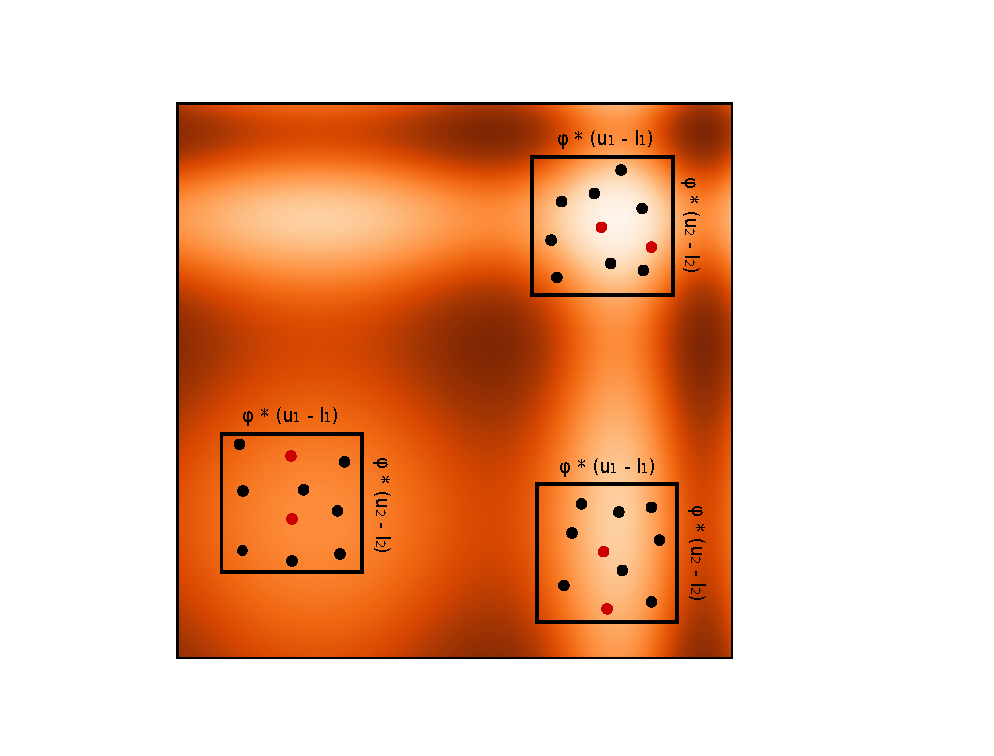
\includegraphics[width=1.1\linewidth]{fig_3.eps}
  \caption{}
  \label{fig:SpaceReduction-b}
\end{subfigure}
\caption{Example showing the application of the space reduction heuristic. In (a) we have the space reduction around the three individuals of Figure 2 ($\bm{x}_1$, $\bm{x}_5$ and $\bm{x}_8$) in red. In (b) are the respective populations generated in each restricted space to apply ITGO, with the local optimal points in red.}\label{fig:SpaceReduction}
\end{figure}


At each iteration, a new population size is set, along with a new value for $K$, which is usually smaller than in the previous iteration.


\subsection{Constrained Optimization}

Until the moment, the ITGO algorithm was presented only for unconstrained optimization problems. ITGO was applied previously to constrained optimization problems \citep{ITGO2, ITGO3}, handling constraints by using a specific local search procedure or by penalizing infeasible individuals.

In this work, we propose a different approach, adopting a mechanism for comparing solutions proposed in \cite{ConHandling}, and used in some very competitive meta-heuristics, specially on differential evolution algorithms \citep{DE1, DE2, DE3}. As in this work we propose a constrained version of ITGO, in the rest of the paper it is named as C-ITGO, standing for Constrained ITGO. The method for comparison comprises the three steps criteria:

\begin{itemize}

\item Between two feasible solutions, the fittest one is better.

\item A feasible solution is always preferred over an infeasible solution, irrespectively of its fitness.

\item Between two infeasible solutions, the one with the smallest sum of constraint violation (equation \ref{eq:viol}) is better.

\end{itemize}


In the topographical heuristic step, we compare two solutions using this three steps criteria with probability $\alpha$, and otherwise, we compare only the fitness value. What we try to achieve with this heuristic is keeping promising solutions with small violation of constraints for further exploration in the local search step.

We generate a symmetric matrix of random numbers $R$, with $R_{i, j} = R_{j, i} \in [0, 1]$. If $R_{i, j} < \alpha$, then we compare elements $\bm{x}_i$ and $\bm{x}_j$ using the three steps criteria. Otherwise, only the fitness value is compared. In general, with this configuration, the number of local optimal points selected by the topographical heuristic is smaller, specially on problems with a small feasible area. 

An important thing to notice is that some distributions of the individuals, with populations of small size and a high value of $K$, may not generate any local optimum in the topographical heuristic. In the case of none of the individuals are selected as local optimum given the current population, we take the best individual according to the three steps criteria as the only local optimum of that population. In practice, however, it is rather unusual to happen.

The best individual in the whole search is always selected using the three steps criteria described above, since feasible solutions are generally preferred. In addition to this new topographical selection method, we also use local search algorithms for constrained optimization.


\subsection{Implementation}

We now present an overview of the implementation of the method, along with pseudocodes describing all necessary steps. Algorithm \ref{alg:ITGO} shows the general procedure for the C-ITGO algorithm.

The parameters are the functions $f(\cdot)$ and $v(\cdot)$, which return the function value and sum of constraints violation respectively, as defined in equations \ref{eq:func} and \ref{eq:viol}, the lower and upper bound vectors $\bm{l}$ and $\bm{u}$, the vector of population sizes $\bm{PS}$, the vector of the $K$ values $\bm{KS}$, the maximum number $Max\_LS$ of elements to execute the local search, the maximum number of function calls allowed in the local search, $LS_1$ and $LS_2$, the space reduction factor $\phi$ and the probability for the three steps comparison $\alpha$.



\documentclass[A4, 11pt, preprint]{elsarticle}

\input{Packages.tex}

\input{BibStyle.tex}



\modulolinenumbers[5]

\journal{Expert Systems with Applications}

\onehalfspacing





\begin{document}



\input{Presentation}


\input{Introduction}


\input{Methods}


\input{Results}


\input{Conclusion}


\input{Acknowledgment}



\setlength{\bibsep}{0pt plus 0.3ex}

\section*{References}

\bibliography{ITGO.bib}



\end{document}


The first line initializes the vector $\bm{best}$ randomly within the range $[\bm{l}, \bm{u}]$, which is the variable that saves the best element found in the search. The main loop starts at line 2, where we check for convergence. The function $Converged$ is problem dependent and may take into account the number of iterations, the number of function calls, the convergence of the best individual or any other stopping criteria.

Line 3 initializes the vector of current populations, with all the $\bm{PS}(1)$ elements inside the bounds of the problem ($[\bm{l}, \bm{u}]$). The set $TopoBest$ at line 4 comprises the best local optimum elements found in all populations and is initialized empty. We use $random$ here to denote the generation of a random scalar or vector for simplicity, although in the implementation we used Sobol sequences for the generation of the individuals.

For each population size (line 5), which is the number of space reductions plus one, we generate new populations, starting from the empty set at line 6. Here, we use $|\cdot|$ to denote the number of elements inside a set or a vector. Line 7 loops through all the populations and execute the topographical heuristic ($TopographicalHeuristic$ function), with $K = \bm{KS}(p)$. The variable $Topo_p$, at line 8, saves the local optimal points selected from the current population.

If the current space reduction is not the last ($p < |\bm{PS}|$, line 9), we create a new population around every point in the $Topo_p$ set, with size $\bm{PS}(p + 1)$ and space reduced at every dimension by $\phi^p$ (lines 10 and 11). Otherwise, if it is the last space reduction, we have to save the local optimal points in the set $TopoBest$ to apply local search (lines 12 and 13).\\[-1em]


\begin{breakablealgorithm}
\caption{CreatePop($\bm{x}$, $\bm{l}$, $\bm{u}$, $popSize$, $\phi$)}
\label{alg:CreatePop}
\begin{algorithmic}[1]

\State $\bm{l}' \gets max(\bm{l}, \bm{x} - (0.5 * \phi) * (\bm{u} - \bm{l}));$
\State $\bm{u}' \gets min(\bm{u}, \bm{x} + (0.5 * \phi) * (\bm{u} - \bm{l}));$
\State $Population \gets \{\bm{x} = \bm{x}^1, ..., \bm{x}^{popSize} : \bm{x} \in random(\bm{l}', \bm{u}')\};$

\State \Return $Population;$




\end{algorithmic}
\algcomment{Create a new population shrinked by $\phi$ around the point $\bm{x}$.}
\end{breakablealgorithm}


The $CreatePop$ procedure is shown in algorithm \ref{alg:CreatePop}. Given an individual $\bm{x}_b$ (a selected local optimum), the function returns a new randomly generated population with $popSize-1$ individuals around this solution, in the original space reduced by the fraction $\phi$. If the point is closer than $0.5 * (u_i - l_i), \ i = 1, ..., n$, from the lower or upper bounds at dimension $i$, the limits of that new population are taken to be the original bounds. The $min$ and $max$ operations are executed element by element. The solution $\bm{x}_b$ is also added to the new population.


At line 14, we check again if the current space reduction is not the last, and update the current populations at line 15, if the condition holds. Line 16 selects the $Max\_LS$ best elements of the set $TopoBest$, using the three steps criteria comparison as sorting criteria. If $|TopoBest| < Max\_LS$, we keep all the elements.

We loop through all the elements of the now sorted $TopoBest$ set at line 17, and apply local search, with at maximum $LS_1$ function evaluations, at line 18. The function $Compare$ (line 19) is the three steps comparison, returning true if the first solution (third argument) is better than the second solution (fourth argument), and returns false otherwise. The element returned by the local search procedure is compared against the best element found in the whole search at line 19. If it is better than the best element found (according to the three steps criteria), or if its fitness is better, a new local search procedure is applied, now with $LS_2$ iterations, at line 20.

%The number of function calls is generally the determining factor of performance, so we wish to make the smallest number of local search iterations as possible since a call for the local search for each individual, in general, does hundreds or thousands of function evaluations.

The number of function calls is usually the determining performance factor. So, we wish to do as few local search iterations as possible, since a call to the local search algorithm typically makes hundreds or thousands of function evaluations. Here, we set $LS_2 > LS_1$, so every element undergoes $LS_1$ function evaluations in the local search, but we only search finely for promising solutions, setting larger values for $LS_2$. Usually, the second local search is only necessary for problems where very finely tuned solutions are required.

At line 21 we compare again the solution generated by the second local search ($\bm{x}$) against the best element found in the whole search ($\bm{best}$) using the three steps criteria. If the new solution is better, we set $\bm{best}$ to that solution at line 22 and continue the loop for applying local search in the other elements. At the end of the execution, when $Converged$ in the outer loop returns true, we return the best solution found in the whole search at line 23. In practice, however, we may stop the algorithm as soon as the optimal solution is found or when the maximum number of function evaluations is reached.

Finally, let us explain the $TopographicalHeuristic$ procedure, shown in algorithm \ref{alg:TopographicalHeuristic}. The function takes as parameters: the objective function $f(\cdot)$ and the sum of constraints function $v(\cdot)$, the current population to be evaluated, the value $K$ for the $KNN$ set, and the probability $\alpha$, for the three steps comparison.


\begin{algorithm*}
\caption{TopographicalHeuristic($f(\cdot)$, $v(\cdot)$, $Population$, $K$, $\alpha$)}
\label{alg:TopographicalHeuristic}
\begin{spacing}{1.5}
\begin{algorithmic}[1]


\State $M \gets |Population|;$
\State $\bm{best} \gets Population(0);$
\State $KNN_K \gets Build\_KNN(Population, K);$
\State $\bm{R} \gets random([0, 1]^{M \times M});$
\State $TopoBest \gets \{\};$
%\State $\bm{Dist}_{i, j} \gets \{|Population(i) - Population(j)|, \ i, j \in \{1, ..., |Population|\}\};$ 

\For{$i \in \{1, ..., |Population|\}$}

\State $insert \gets \bm{True};$

\For{$j \in \{1, ..., |Population|\} \ \cap \ \{\bm{x}_j \in KNN_K(\bm{x}_i)\}$}
	\If{$\bm{R}_{i, j} < \alpha$}
		\State $insert \gets insert$ \& $Compare(f(\cdot), v(\cdot), \bm{x}_i, \bm{x}_j);$
	\Else
		\State $insert \gets insert$ \& ($f(\bm{x}_i) < f(\bm{x}_j));$
	\EndIf
\EndFor

\If{$insert = \bm{True}$}
\State $TopoBest \gets TopoBest \ \cup \ \{\bm{x}_i\};$
\EndIf

\If{$Compare(f(\cdot), v(\cdot), \bm{x}_i, \bm{best})$}
\State $\bm{best} \gets \bm{x}_i;$
\EndIf
\EndFor

\If{$|TopoBest| = 0$}
	\State $TopoBest \gets \{\bm{best}\};$
\EndIf

\State \Return $TopoBest;$



\end{algorithmic}
\end{spacing}
\algcomment{Topographical heuristic procedure.}
\end{algorithm*}


Lines 1-5 simply initialize the necessary structures. Namely, the number of elements $M$ in $Population$, the $\bm{best}$ vector, which is the best element of the entire population based on three steps comparison (initially set to any individual of the population), the $KNN_K$ structure based on the elements of the population, which is a mapping from a solution vector $\bm{x}$ to a set of the vectors that belong to the $KNN_K$ of $\bm{x}$, the random symmetric matrix $R$, with every element in the range $[0, 1]$, and the $TopoBest$ set, containing the local optimal points, initially empty.

At line 6 we loop through all indices of $Population$, and set the $insert$ flag to $\bm{True}$ at line 7, which indicates if the individual $\bm{x}_i$ is a local optimal point. For every index $j$, such that $\bm{x}_j$ is in the set $KNN_K(\bm{x}_i)$ (line 8), we compare $\bm{x}_j$ with $\bm{x}_i$. If $R_{i, j} < \alpha$, then we set the flag $insert$ to the boolean result of applying the \textit{and} operator ($\&$) to $insert$ and the result of $Compare$ (lines 9-10). That is, if $Compare$ returns false at least one time for any $j$, $insert$ will also be false for the index $i$. If $R_{i, j} >= \alpha$, then we execute the same procedure, but now using fitness only comparison, at lines 11-12.

At line 13 we check if $insert = \bm{True}$, and, if so, $\bm{x}_i$ is a local optimum, and we insert it in the $TopoBest$ set, at line 14. Lines 15-16 select the best element found in the whole population based on the three steps comparison, and stores that solution in the variable $\bm{best}$. In case of no solution is selected as a local optimum, the set $TopoBest$ is composed only of the $\bm{best}$ element (lines 17-18). At line 19 we return the $TopoBest$ set, containing all the local optimal points (or the $\bm{best}$ element).


\subsection{Local Search}

In this section, we discuss the three different methods of local search used in C-ITGO and their implications on the final performance.

As we used Matlab to program C-ITGO, a natural choice for local search is the optimization toolbox. In the case of real non-linearly constrained problems, we used the \textit{SQP} (Sequential Quadratic Programming), present in the \textit{fmincon} package \citep{fmincon}. The basic SQP algorithm is described in Chapter 18 of \cite{Nocedal}, although the actual implementation used in fmincon uses some additional heuristics. 

A very successful method, also implemented in Matlab, that uses that same package (SQP of fmincon) is the \textit{MVMO} (Mean-Variance Mapping Optimization) \citep{MVMO}, winner of two different categories of the IEEE Congress on Evolutionary Computation competition on real optimization in 2016.

For mixed integer problems with nonlinear constraints, we used the \textit{OPTI} toolbox \citep{OPTI}, which has many algorithms specialized for mixed integer programming. Specifically, we used the \textit{BONMIN} (Basic Open-source Nonlinear Mixed INteger programming) \citep{BONMIN} and the \textit{NOMAD} (Nonlinear optimization with the MADS algorithm) \citep{NOMAD} solvers.

We emphasize here that any kind of local search can be used in conjunction with C-ITGO. We could use for example a specialized local search for a given problem. In this work, both problems on continuous and integer domains are treated in the same way, changing only the local search procedure.

It is true that some simpler problems can be solved solely by using an exact method such as those cited above, for example by calling the procedure at different random points. However, in multimodal objective functions with nonlinear constraints, it is usually not possible to find the global optimum. And even if a problem can be solved by an exact method, the number of function evaluations might be very large.

The objective is not to rely heavily on the local search procedure. Rather, what we want to achieve with the topographical heuristic is provide solutions close to a local or global optimum, so that any reasonably good local search can converge with relative ease. In this work, the maximum number of function evaluations allowed in the first call to the local search procedure is kept as small as possible, and, in most cases, it is enough to find optimal or nearly optimal solutions.



\subsection{Parameters}

Given the differences in the number of variables, constraints, size of the space, number of function calls to converge reported by competing methods, and general complexity of the problems considered in this work, we selected experimentally specific parameters for each problem aiming to obtain the best performance of C-ITGO. This is a general approach taken for most of the optimization methods compared here. The parameters were selected so as to find optimal or near-optimal solutions while minimizing the number of function evaluations (NFEs).

Table \ref{tab:Parameters} shows the choice of the parameters for the eight engineering design problems we consider: Welded Beam (WB), Tension/Compression Spring (TC), Three-Bar truss (TB), Speed Reducer (SRI and SRII), Pressure Vessel (PV), Gear Train (GT) and Multiple Disk clutch brake (MD). We will comment each problem and the results obtained by C-ITGO and other competing methods in Section \ref{sec:Results}.


\begin{table*}[tp]
    \tiny
\begin{center}
\begin{tabular}{ | P{0.8cm} | P{0.8cm} | P{0.8cm} | P{0.8cm} | P{0.8cm} | P{0.8cm} | P{0.8cm} | P{0.8cm} | P{0.8cm} | P{0.9cm} | P{0.9cm}  | }
\hline
$\bm{Prob / \allowbreak Param}$ & $\bm{PS_1}$ & $\bm{PS_2}$ & $\bm{K_1}$ & $\bm{K_2}$ & $\bm{\alpha}$ & $\bm{\phi}$ & $\bm{LS1}$ & $\bm{LS2}$ & $\bm{MaxLS}$ & $\bm{LSType}$ \\
\hline

\textbf{WB} & 100 & 10 & 10 & 3 & 0.5 & 0.2 & 100 & 200 & 5 & \textbf{SQP} \\
\textbf{TC} & 50 & 10 & 8 & 3 & 0.5 & 0.2 & 100 & 200 & 5 & \textbf{SQP} \\
\textbf{TB} & 30 & 5 & 5 & 2 & 0.5 & 0.2 & 20 & 70 & 5 & \textbf{SQP} \\
\textbf{SRI} & 150 & 10 & 10 & 3 & 0.5 & 0.2 & 100 & 200 & 5 & \textbf{BONMIN} \\
\textbf{SRII} & 100 & 10 & 10 & 3 & 0.5 & 0.2 & 50 & 100 & 5 & \textbf{SQP} \\
\textbf{PV} & 50 & 10 & 8 & 3 & 0.5 & 0.5 & 30 & 100 & 5 & \textbf{BONMIN} \\
\textbf{GT} & 20 & 5 & 5 & 2 & 0.5 & 0.7 & 30 & 100 & 5 & \textbf{NOMAD} \\
\textbf{MD} & 20 & 5 & 7 & 2 & 0.5 & 0.7 & 100 & 200 & 5 & \textbf{NOMAD} \\
\hline

\end{tabular}
\end{center}
\vspace*{-6mm}
\caption{Parameters of C-ITGO for each engineering design problem.. \\[1em]}
\label{tab:Parameters}
\end{table*}



For all problems, we only use a single space reduction, which generates two populations and two values for $K$, namely $PS_1$ (first population size, before space reduction) and $PS_2$ (second population size, after space reduction), $K_1$ and $K_2$ (also before and after space reduction, respectively). The value for the probability $\alpha$ was kept constant for all problems, as well as the maximum number of elements to execute the local search, $MaxLs$. The value of $\phi$ was set to smaller values for problems defined on entirely continuous domains and assumed higher values for mixed integer problems. The $LS_1$ and $LS_2$ control the maximum number of allowed function evaluations in the local search in the first and second calls, respectively. Finally, $LSType$ represents the algorithm used in the local search. %In next section, we discuss the three different methods of local search used and their implications on the final performance of the method.

The type of local search was determined based on the properties of each problem. For problems with only continuous variables, we used the SQP method (WB, TC, and TB). For problems with only discrete variables, we used the NOMAD solver (GT, MD), and for mixed integer problems, we used the BONMIN solver (SRI and PV). The only exception was SRII, in which we used the SQP algorithm rounding the variables that are required to be an integer. In tests with this specific problem, it resulted in better solutions than using the mixed integer solvers.


\section{Computational Results} \label{sec:Results}

To evaluate the performance of the developed method, we use eight difficult constrained engineering optimization problems, including continuous and mixed integer problems. We now present a general overview of each problem, along with comparison with state of the art results.

In all tests, we run CI-TGO 25 times, saving the best and worst feasible solutions, as well as the mean value and standard deviation of the fitness after all runs. Given the great variability between the results found in literature for most problems, we stop the execution of CI-TGO as soon as the best found solution in a run is considerable close to the optimum. Also, a fixed number of maximum number of function evaluations was set for each problem. If the number of FEs exceeds this number, the algorithm immediately stops, and the best found solution is returned. At the end, the average number of function calls is reported for all runs.

In our tests, all solutions reported by CI-TGO are completely feasible, for all problems, so we exclude from comparison methods that violate any constraint.

We compare 27 different optimization against CI-TGO. In order of presentation, they are: PSO-DE \cite{PSO-DE}


\subsection{Welded bean design problem}

The welded bean design \citep{WB} is the problem of minimizing the fabrication cost of a welded bean, subject to seven inequality constraints, being two linear and five non linear. The constraints include shear stress, bending stress in the beam, buckloading on the bar and end deflection on the beam. The four design variables are continuous. Figure \ref{fig:WB} shows the structure of the problem.

\begin{figure}[h]
\begin{center}
\includegraphics[scale=0.7]{Imgs/WB.jpg}
\end{center}
\captionsetup{justification=centering}
\caption{Welded bean design problem structure.}\label{fig:WB}
\end{figure}

We compare the results obtained by CI-TGO against a number of state of the art methods used to solve this problem, including PSO-DE, HPSO, MBA, CPSO, LCA, NM-PSO, IABC-MAL, IAPSO and SAMP-Jaya. Table \ref{tab:WB} shows the comparison of the results obtained by all cited methods to solve the welded bean design problem. All the methods, with exception of SAMP-Jaya and CI-TGO, took more than 10,000 iterations to achieve good quality solutions. CI-TGO achieved optimal solutions with a very small standard deviation of $6.7E \!-\! 16$ with ten times less function evaluations in average than most of the methods.


\begin{table*}[tp]
    \tiny
\begin{center}

\begin{tabular}{ P{2.0cm} P{2.0cm} P{2.0cm} P{2.0cm} P{2.0cm} P{2.0cm} P{2.0cm} P{2.0cm}  }
\hline
\textbf{Method} & \textbf{Best} & \textbf{Mean} & \textbf{Worst} & \textbf{SD} & \textbf{MNFEs} \\
\hline
PSO-DE & 1.724852 & 1.724852 & 1.724852 & 6.70E-16 & 66,600 \\
HPSO & 1.724852 & 1.814295 & 1.749040 & 4.01E-02 & 81,000 \\
UPSO & 1.921990 & 2.837210 & N/A & 6.83E-01 & 100,000 \\
MBA & 1.724853 & 1.724853 & 1.724853 & 6.94E-19 & 47,340 \\
CMA-ES & 1.7248523 & 1.7248523 & 1.7248523 & 1.66E-09 & 4,658 \\
MVDE & 1.7248527 & 1.7248621 & 1.7249215 & 7.88E-06 & 15,000 \\
CPSO & 1.728024 & 1.748831 & 1.782143 & 1.29E-02 & 240,000 \\
LCA & 1.7248523 & 1.7248523 & 1.7248523 & 7.11E-15 & 15,000 \\
IPSO & 1.724852 & 1.7248787 & 1.7250002 & 3.28E-05 & 20,000 \\
CB-ABC & 1.724852 & 1.724852 & N/A & 2.38E-11 & 15,000 \\
DELC & 1.724852 & 1.724852 & 1.724852 & 4.10E-13 & 20,000 \\
IABC-MAL & 1.724852 & 1.724852 & 1.724852 & 2.31E-12 & 15,000 \\
NM-PSO & 1.724717 & 1.726373 & 1.733393 & 3.50E-03 & 80,000 \\
APSO & 1.736193 & 1.877851 & 1.993999 & 0.076118 & 50,000 \\
WCA & 1.724856 & 1.726427 & 1.744697 & 4.29E-03 & 46,450 \\
IAPSO & 1.7248523 & 1.7248528 & 1.7248624 & 2.02E-06 & 12,500 \\
SAMP-Jaya & 1.724852 & 1.724852 & 1.724852 & 6.7E-16 & 3,618.25 \\
\textbf{C-ITGO} & \bf{1.7248523} & \bf{1.7248523} & \bf{1.7248523} & \bf{3.65E-12} & \bf{940.68} \\


\hline
\end{tabular}
\end{center}
\vspace*{-6mm}
\caption{Statistical results of different methods for Welded beam problem. \\[1em]}
\label{tab:WB}
\end{table*}



The results for CI-TGO and SAMP-Jaya are very similar, with same standard deviation, but with the former converging in less than one third of the number of function evaluations. We note here that the best solution achieved by NM-PSO is slightly infeasible, so it should not be directly compared to the rest of the methods.




\subsection{Tension / compression spring design problem}

This problem was introduced by \cite{TC}, and the objective is the minimization of the weight of a tension / compression string (Figure \ref{fig:TC}). The problem has three continuous design variables, being them the diameter of spring wire, the diameter of spring mean coil and the number of active coils. It is subject to three non linear and one linear inequality constraints.

\begin{figure}[h]
\begin{center}
\includegraphics[scale=0.6]{Imgs/TC.png}
\end{center}
\captionsetup{justification=centering}
\caption{Schematic view of the tension/compression spring design problem}\label{fig:TC}
\end{figure}


A variety of methods were used in literature to solve the tension / compression spring design problem. Between them, we can cite HPSO, NM-PSO, MBA, PSO-DE, ABC, PSO, CB-ABC, CPSO, GA1, GA2, QPSO, G-QPSO, CAEP, DELC, IAPSO, IABC-MAL and SAMP-Jaya. Table \ref{tab:TC} shows the statistical results of all methods, along with the number of function evaluations taken to achieve such results.


\begin{table*}[tp]
    \tiny
\begin{center}

\begin{tabular}{ P{2.0cm} P{2.0cm} P{2.0cm} P{2.0cm} P{2.0cm} P{2.0cm} P{2.0cm} P{2.0cm}  }
\hline
\textbf{Method} & \textbf{Best} & \textbf{Mean} & \textbf{Worst} & \textbf{SD} & \textbf{NFEs} \\
\hline

HPSO & 0.012665 & 0.012719 & 0.012707 & 1.58E-05 & 81,000 \\
NM-PSO & 0.012630 & 0.012633 & 0.012631 & 8.47E-07 & 80,000 \\
MBA & 0.012665 & 0.012713 & 0.012900 & 6.30E-05 & 7,650 \\
PSO-DE & 0.012665 & 0.012665 & 0.012665 & 1.20E-08 & 24,950 \\
ABC & 0.012665 & N/A & 0.012709 & 1.28E-02 & 30,000 \\
PSO & 0.012857 & 0.071802 & 0.019555 & 1.16E-02 & 2,000 \\
CB-ABC & 0.012665 & 0.012671 & N/A & 1.42E-05 & 15,000 \\
CPSO & 0.012675 & 0.012924 & 0.012730 & 5.20E-04 & 240,000 \\
GA1 & 0.012704 & 0.012769 & 0.012822 & 3.94E-05 & 900,000 \\
GA2 & 0.012681 & 0.012742 & 0.012973 & 5.9E-0.5 & 80,000 \\
QPSO & 0.012669 & 0.018127 & 0.013854 & 1.34E-03 & 2,000 \\
G-QPSO & 0.012665 & 0.017759 & 0.013524 & 1.27E-03 & 2,000 \\
CAEP & 0.012721 & 0.015116 & 0.013568 & 8.42E-04 & 50,020 \\
DELC & 0.012665 & 0.012666 & 0.012665 & 1.30E-07 & 20,000 \\
IAPSO & 0.01266523 & 0.013676527 & 0.01782864 & 1.573E-3 & 2,000 \\
IABC-MAL & 0.01266523 & 0.01266525 & 0.01266539 & 6.78E-08 & 15,000 \\
SAMP-Jaya & 0.012664 & 0.013193 & 0.012714 & 9.25E-05 & 6,861 \\
CI-TGO & 0.01266523 & 0.01266523 & 0.01266525 & 2.81E-9 & 535.08 \\

\hline
\end{tabular}
\end{center}

\caption{\fnt{8} Tension Compression. \\[1em]}
\label{tab:TC}
\end{table*}




The methods vary greatly in the number of function evaluations required to converge to good quality solutions. Only four of the methods (PSO, QPSO, G-QPSO and IAPSO) achieved convergence with 2,000 function evaluations, while some methods required more than 100,000. The best solution achieved by all methods have the same fitness value up to 3 decimal places.
 
The best solution reported by NM-PSO is again infeasible, so we do not compare it against other methods. The SAMP-Jaya method also seems to report a slightly infeasible best found solution, differing from the optimal value reported by other methods. However, the result differs only at the sixth decimal place, and the difference may be due to wrong rounding. We cannot state this for sure since we do not have access to the solution vector found by the method. Given the differences in rounding between the methods, we consider $f(\bm{x}) = 0.012665$ to be the best found solution.

The CI-TGO method performed remarkably well on this problem, converging to the best found solution among all methods in 535.08 function evaluations on average, almost four times less than the second competing method. Also, the standard deviation is very small, in the order of $2.81E-9$. 

Given the relatively small domain of the problem, we believe that the CI-TGO method was able to cover the space efficiently, providing hot starting points for the local search method, which proved to be very effective in this case.




\subsection{Three-bar truss design problem}

The three-bar truss design problem \citep{TB} consists in minimizing the volume of a statically loaded three-bar truss. Theere are two continuous design variables and three non linear inequality constraints, based on the stress ($\sigma$) on each of the truss members. Figure \ref{fig:TB} shows the schematic view of the problem.

\begin{figure}[h]
\begin{center}
\includegraphics[scale=0.5]{Imgs/TB.png}
\end{center}
\captionsetup{justification=centering}
\caption{Structure of three-bar truss design problem}\label{fig:TB}
\end{figure}


Here we present only the five good performing methods used to solve this problem, since the solutions found in literature have very small variance from each other. These methods are CMA-ES, MVDE, DELC, MBA and IABC-MAL. We present the statistical results for this problem in table \ref{tab:TB}.


\begin{table*}[tp]
    \tiny
\begin{center}

\begin{tabular}{ P{2.0cm} P{2.0cm} P{2.0cm} P{2.0cm} P{2.0cm} P{2.0cm} P{2.0cm} P{2.0cm}  }
\hline
\textbf{Method} & \textbf{Best} & \textbf{Mean} & \textbf{Worst} & \textbf{SD} & \textbf{MNFEs} \\
\hline

CMA-ES & 263.895843 & 263.895843 & 263.895843 & 2.7E-09 & 1,706 \\
MVDE & 263.895843 & 263.895843 & 263.895855 & 2.58E-07 & 7,000 \\
DELC & 263.895843 & 263.895843 & 263.895843 & 4.3E-14 & 10,000 \\
MBA & 263.895852 & 263.897996 & 263.915983 & 3.93E-03 & 13,280 \\
IABC-MAL & 263.895843 & 263.895843 & 263.895843 & 0.0 & 15,000 \\
C-ITGO & 263.895843 & 263.895843 & 263.895843 & 2.0E-12 & 136.48 \\


\hline
\end{tabular}
\end{center}

\caption{\fnt{8} Statistical results of different methods for three-bar truss design problem. \\[1em]}
\label{tab:TB}
\end{table*}



We can note that all methods have very similar results, differing mainly in the number of function calls. This is not surprising, given that the problem is simpler, has less variables and has a smaller domain than any other problem used in this work.

CI-TGO achieved convergence quickly, taking 141.8 function evaluations in average. In this problem, we have set a small population, as well as small number of function calls allowed in the local search procedure. It seems that the solutions found by the topographical heuristic were already close to the optimum, so the local search converged in very few iterations. However, the CI-TGO method still has a worst standard deviation than DELC and IABC-MAL.





\subsection{Speed reducer design problem}

The total weight of the speed reducer (Figure \ref{fig:SR}) is to be minimized. The problem has seven design variables: face width, teeth module, number of teeth on pinion, first and second length of shafts between bearings and first and second shafts diameter \citep{SR}. The problem has 11 non linear constraints, and the third variable is constrained to be integer. We use two versions of this problem, where the only difference is in the bounds of the fifth variable. We will call this problems SRI and SRII, respectively.


\begin{figure}[h]
\begin{center}
\includegraphics[scale=0.6]{Imgs/SR.jpg}
\end{center}
\captionsetup{justification=centering}
\caption{Schematic view of the speed reducer design problem}\label{fig:SR}
\end{figure}

For SRI, we compare CI-TGO results against 5 optimization methods, namely COPSO, LCA, CiP-PSO, IPSO and IAPSO, shown in table \ref{tab:SP1}. The reported results for the SAMP-Jaya method seems to violate the integer constraint at variable three, so we do not include it in our comparison. The LCA, IPSO, IAPSO and CI-TGO present similar results, all finding the global optimum solution and having very low standard deviation. The SiC-PSO and COPSO methods present inferior results, with higher average fitness. Besides having significant difference between the best from the mean fitness value, the SiC-PSO reports a standard deviation of 0.


\begin{table*}[tp]
    \tiny
    \begin{center}
    
    \begin{tabular}{ P{2.0cm} P{2.0cm} P{2.0cm} P{2.0cm} P{2.0cm} P{2.0cm} P{2.0cm} P{2.0cm}  }
    \hline
    \textbf{Method} & \textbf{Best} & \textbf{Mean} & \textbf{Worst} & \textbf{SD} & \textbf{NFEs} \\
    \hline
    
    SiC-PSO & 2996.34816 & 2996.4085 & NA & 0.0 & 24,000 \\
    COPSO & 2996.372448 & 2996.408525 & NA & 2.867E-02 & 30,000 \\
    LCA & 2996.34816497 & 2996.34816497 & 2996.34816497 & 2.63E-12 & 24,000 \\
    IPSO & 2996.34816497 & 2996.3481 & 2996.34816509 & 2.43E-18 & 20,000 \\
    IAPSO & 2996.34816497 & 2996.34816497 & 2996.34816497 & 6,88E-13 & 6,000 \\
    CI-TGO & 2996.34816497 & 2996.34816497 & 2996.34816497 & 7.5E-13 & 856.40 \\
        
    \hline
    \end{tabular}
    \end{center}
    
    \caption{\fnt{8} SP1. \\[1em]}
    \label{tab:SP1}
    \end{table*}
    
    

The first four methods take more than 20,000 iterations to converge to good quality solutions, while IAPSO takes only 6,000 FEs. CI-TGO outperforms the other methods by a large margin, converging in 858.40 function calls in average, while maintaining negligible worst standard deviation than IAPSO and IPSO.

For this problem, we used considerable greater populations, of sizes 150 and 10, while maintaining the number of allowed function evaluations of the local search relatively small (100 and 200). For the worst case, CI-TGO takes 3 full iterations to converge, while converging in the first iteration in most runs.

For SRII, the methods used for comparison were PSO-DE, MBA, DELC, CB-ABC, CMA-ES, IABC-MAL, IPSO and IAPSO. From Table \ref{tab:SP2}, we can see that DELC, CMA-ES, IAPSO and CI-TGO are the only methods that converged very close to the optimum in every run, having very small standard deviation. Although similar results are observed regarding the quality of the solutions, CI-TGO converges much quicker than any competing method, using six times less function evaluations than IAPSO. The standard deviation achieved by CI-TGO is also the smallest among all compared methods.


\begin{table*}[tp]
    \tiny
    \begin{center}
    
    \begin{tabular}{ P{2.0cm} P{2.0cm} P{2.0cm} P{2.0cm} P{2.0cm} P{2.0cm} P{2.0cm} P{2.0cm}  }
    \hline
    \textbf{Method} & \textbf{Best} & \textbf{Mean} & \textbf{Worst} & \textbf{SD} & \textbf{MNFEs} \\
    \hline
    
    PSO-DE & 2996.348167 & 2996.348174 & 2996.348204 & 6.40E-06 & 54,350 \\
    MBA & 2994.482453 & 2996.769019 & 2999.652444 & 1.56E+00 & 6,300 \\
    DELC & 2994.471066 & 2994.471066 & 2994.471066 & 1.90E-12 & 30,000 \\
    CB-ABC & 2994.471066 & 2994.471066 & N/A & 2.48E-07 & 15,000 \\
    CMA-ES & 2994.471066 & 2994.471066 & 2994.471066 & 8.98E-10 & 12,998 \\
    IPSO & 2994.471067 & 2994.47108 & 2994.4711 & 9.27E-06 & 20,000 \\
    IAPSO & 2994.471066 & 2994.471066 & 2994.471066 & 2.65E-09 & 6,000 \\
    CI-TGO & 2994.471066 & 2994.471066 & 2994.471066 & 9.28E-13 & 906.32 \\ 
    
  

    \hline
    \end{tabular}
    \end{center}
    
    \caption{\fnt{8} Statistical results of different methods for the speed reducer design problem II. \\[1em]}
    \label{tab:SP2}
    \end{table*}
    
    

For this specific problem, we used the SQP algorithm as local search, and rounded the value of the third variable. In this case, this approach proved to converge much faster than using a mixed integer local search. Also, the first population size is considerable smaller than the one used in SRI (100 in this problem).



\subsection{Pressure vessel design problem}

In the pressure vessel design problem, the objective is to minimize the total manufacturing cost, including the cost of the material, forming and welding costs \citep{PV}. The problem is subject to three linear and one non linear inequality constraint, and its structure is shown in Figure \ref{fig:PV}. The four variables are the thickness of the shell, the thickness of the head, the inner radius, and the length of the cylindrical section of the vessel. This is an example of a mixed integer problem, where the first and second variables are constrained to be integers.


\begin{figure}[h]
\begin{center}
\includegraphics[scale=0.6]{Imgs/PV.png}
\end{center}
\captionsetup{justification=centering}
\caption{Pressure vessel design problem structure.}\label{fig:PV}
\end{figure}


Some methods in literature optimized the pressure vessel design problem without taking into account the integer constraints at the first and second variables. So, to compare the CI-TGO performance against other methods, we will only consider methods that respect the integer constraints.


\begin{table*}[tp]
    \tiny
    \begin{center}
    
    \begin{tabular}{ P{2.0cm} P{2.0cm} P{2.0cm} P{2.0cm} P{2.0cm} P{2.0cm} P{2.0cm} P{2.0cm}  }
    \hline
    \textbf{Method} & \textbf{Best} & \textbf{Mean} & \textbf{Worst} & \textbf{SD} & \textbf{MNFEs} \\
    \hline
    
    QPSO & 6059.7209 & 8017.2816 & 6440.3786 & 4.79E+02 & 8,000 \\
    G-QPSO & 6059.7208 & 7544.4925 & 6440.3786 & 4.48E+02 & 8,000 \\
    CMA-ES & 6059.7143 & 6170.25055 & 6410.08676 & 140.4843 & 30,018 \\
    MVDE & 6059.7144 & 6059.99724 & 6090.53353 & 2.9103 & 15,000 \\ 
    CB-ABC & 6059.7143 & 6126.6237 & NA & 1.14E+02 & 15,000 \\
    HPSO & 6059.7143 & 6099.9323 & 6288.6770 & 86.2000 & 81,000 \\
    WCA & 5885.3327 & 6198.6172 & 6590.2129 & 213.0490 & 27,500 \\
    LCA & 6059.8553 & 6070.5884 & 6090.6114 & 11.37534 & 24,000 \\
    APSO & 6059.7242 & 6470.7156 & 7544.4927 & 326.9688 & 200,000 \\
    MBA & 5889.3216 & 6200.64765 & 6392.5062 & 160.34 & 70,650 \\    
    IABC-MAL & 6059.7143 & 6072.5972 & 6089.2720 & 1.88E-06 & 15,000 \\
    SAMP-Jaya & 5872.2129 & 5872.2129 & 5872.2129 & 5.0E-12 & 6513.33 \\    
    IAPSO & 6059.7143 & 6068.7539 & 6090.5314 & 14.0057 & 7,500 \\
    C-ITGO & 6059.7143 & 6059.7143 & 6059.7143 & 9.8E-13 & 1101.64 \\
    
    \hline
    \end{tabular}
    \end{center}
    \vspace*{-6mm}
    \caption{Statistical results of different methods for the pressure vessel design problem. \\[1em]}
    \label{tab:PV}
    \end{table*}
    
    

We compare CI-TGO against the PSO, GA1, GA2, QPSO, G-QPSO, CB-ABC, IABC-MAL and IAPSO methods. The statistical results are shown in table \ref{tab:PV}. The algorithms CB-ABC, IABC-MAl, IAPSO and CI-TGO are the only who found the optimal solution, and also the ones with smaller mean fitness value. All other methods presented relatively poor performance, with much higher FEs in average.

CI-TGO takes less than six times the number of function evaluations to converge than the best competing method, IAPSO, which reported a result of 7,500 FEs. Also, CI-TGO achieves a extremely small standard deviation of $9.8E-13$, many orders of magnitude smaller than IAPSO. All runs of CI-TGO converged quickly to the global optimum, showing unarguably better results than any other method used for comparison in this work.



\subsection{Gear train design problem}

In this problem, the objective is to minimize the cost of the gear ratio of the gear train \citep{PV}. An example is shown in Figure \ref{fig:GT}. The problem has four variables, representing the number of teeth for the four gears. The only constraint of the problem is that all variables must be integers.


\begin{figure}[h]
\begin{center}
\includegraphics[scale=0.6]{Imgs/GT.jpg}
\end{center}
\captionsetup{justification=centering}
\caption{Pressure vessel design problem structure.}\label{fig:GT}
\end{figure}


We compare the CI-TGO results, shown in table \ref{fig:GT}, against other five methods: CS, APSO, MBA, UPSO and IAPSO. In general, all methods compared achieved similar results, having found the optimal solution for the problem. UPSO failed at finding some solutions, while APSO has a considerable greater mean value than other the methods.
The main difference relies in the number of function calls, varying from 100,00 for UPSO to 800, for IAPSO and CI-TGO.


\begin{table*}[tp]
    \tiny
\begin{center}

\begin{tabular}{ P{2.0cm} P{2.0cm} P{2.0cm} P{2.0cm} P{2.0cm} P{2.0cm} P{2.0cm} P{2.0cm}  }
\hline
\textbf{Method} & \textbf{Best} & \textbf{Mean} & \textbf{Worst} & \textbf{SD} & \textbf{NFEs} \\
\hline

MBA[12] & 2.700857E-12 & 2.062904E-08 & 2.471635E-09 & 3.94E-09 & 1120 \\
UPSO[63] & 2.700857E-12 & 3.80562E-08 & N/A & 1.09E-07 & 100,000 \\
CS[62] & 2.7009E-12 & 1.9841E-9 & 2.3576E-9 & 3.5546E-9 & 5,000 \\
APSO[34]* & 2.700857E-12 & 4.781676E-07 & 7.072678E-06 & 1.44E-06 & 8,000 \\
IAPSO & 2.700857E-12 & 5.492477E-09 & 1.827380E-08 & 6.36E-09 & 800 \\
CI-TGO & 2.700857E-12 & 4.6504232E-09 & 2.7264505E-08 & 6.85E-09 & 773.0 \\


\hline
\end{tabular}
\end{center}

\caption{\fnt{8} Statistical results of different methods for the gear train design problem. \\[1em]}
\label{tab:GT}
\end{table*}




Since this is a integer optimization problem, we used the mixed integer local search based on the NOMAD solver. In this problem, the solver had some difficulty in some runs, achieving $6.85E-09$ standard deviation, more than IAPSO, CS and MBA. The mean fitness value, however, is only worst than the MBA method, which takes 1120 function calls to converge. Besides these drawbacks, CI-TGO converges faster than the other methods compared here, taking only 773.0 function calls on average.



\subsection{Multiple disk clutch brake design problem}

This is also an example of a problem where all variables are discrete. The Multiple disk clutch brake design problem aims at minimizing the mass of a multiple disc clutch brake \cite{MD}. There are five integer variables: the inner radius, outer radius, thickness of the disc, actuating force and number of friction surfaces (Figure \ref{fig:MD}). The problem is also constrained by nine non linear inequalities.

\begin{figure}[h]
\begin{center}
\includegraphics[scale=0.6]{Imgs/MD.jpg}
\end{center}
\captionsetup{justification=centering}
\caption{Schematic view of the multiple disk clutch brake design problem.}\label{fig:MD}
\end{figure}

To compare the results, we used only methods who achieved close performance to the obtained by CI-TGO, since some methods in literature have very diverging results. The WCA, IPSO and IAPSO methods achieved good performance in this problem, finding the optimal solution and having very small variance, as shown in table \ref{tab:MD}. The WCA and IAPSO took very few function evaluations to converge, respectively 500 and 400. IPSO took long more, with 20,000 function evaluations. However, the reported standard deviation for IPSO was 0.0.


\begin{table*}[tp]
    \tiny
    \begin{center}
    
    \begin{tabular}{ P{2.0cm} P{2.0cm} P{2.0cm} P{2.0cm} P{2.0cm} P{2.0cm} P{2.0cm} P{2.0cm}  }
    \hline
    \textbf{Method} & \textbf{Best} & \textbf{Mean} & \textbf{Worst} & \textbf{SD} & \textbf{NFEs} \\
    \hline

    WCA & 0.313656 & 0.313656 & 0.313656 & 1.69E-16 & 500 \\
    IPSO & 0.313656 & 0.313656 & 0.313656 & 0.0 & 20,000 \\
    IAPSO & 0.313656 & 0.313656 & 0.313656 & 1.13E-16 & 400 \\
    CI-TGO & 0.313656 & 0.313656 & 0.313656 & 1.13E-16 & 286.48 \\

    \hline
    \end{tabular}
    \end{center}
    
    \caption{\fnt{8} Multiple Disk. \\[1em]}
    \label{tab:MD}
    \end{table*}
    
    

The CI-TGO clearly outperforms the other methods, having a standard deviation of $1.13E-16$, while converging with only 286.48 function evaluations on average. For this problem, we also have used a very small populations, of size 20 and 5. The number of function evaluations in the first step was 100, and most runs converged in much less, enjoying the quality of initial solutions provided by the topographical heuristic step. Some runs, however, took more than 1,500 function evaluations, bringing the mean FEs up.






\iffalse

\begin{align*}
\textbf{Minimize:} & \\
& f(\bm{x}) = 1.10471x_1^2x_2 + 0.04811x_3x_4(14 + x_2) \\[0.5em]
\textbf{subject to:} & \\
& g_1(\bm{x}) = \tau(\bm{x}) - 13,600 \leq 0 \\
& g_2(\bm{x}) = \sigma(\bm{x}) - 30,000 \leq 0 \\
& g_3(\bm{x}) = x_1 - x_4 \leq 0 \\
& g_4(\bm{x}) = 0.10471x_1^2 + 0.04811x_3x_4(14+x_2) - 5  \leq 0 \\
& g_5(\bm{x}) = 0.125 - x_1 \leq 0 \\
& g_6(\bm{x}) = \delta(\bm{x}) - 0.25 \leq 0 \\
& g_7(\bm{x}) = 6,000 - Pc(\bm{x}) \leq 0 \\[0.5em]
\textbf{where:} & \\
& \tau(\bm{x}) = \sqrt{\tau^2 + \frac{(2 \tau' \tau'' x_2)}{2R} + \tau''^2 } \\
& \tau' = \frac{6,000}{(sqrt{2} x_1 x_2)} \\[0.5em]
& \tau'' = \frac{(M R)}{J} \\
& M = 6,000 (14 + \frac{x_2}{2}) \\
& R = sqrt{\frac{x_2^2}{4} + (x_1 + \frac{x_3}{2})^2} \\
& J = 2 x_1 x_2 \sqrt{2} (\frac{x_2^2}{12} + (x_1 + \frac{x_3}{2})^2) \\[0.5em]
& \sigma(\bm{x}) = 504,000 / (x_4 x_3^2) \\
& \delta(\bm{x}) = \frac{65,856,000}{(30 \times 10^6 x_4 x_3^3)} \\
& Pc(\bm{x}) = \frac{4.013(30 \times 10^6)}{196} \sqrt{x_3^2 \frac{x_4^6}{36}} \Bigg(1 - \frac{x_3}{28} \sqrt{\frac{30 \times 10^6}{4(12 \times 10^6)}}\Bigg) \\[0.5em]
\textbf{with bounds:} & \\
&  0.1 \leq x_1, x_4 \leq 2 \\
&  0.1 \leq x_2, x_3 \leq 10
\end{align*}

\begin{equation*}
\begin{aligned}
%& \textbf{Minimize:} \\
& f(\bm{x}) = 0.6224z_1x_3x_4 + 1.7781z_2x_3^2 + 3.1661z_1^2x_4 + 19.84z_1^2x_3 \\[0.5em]
& \textbf{subject to:}\\
& g_1(\bm{x}) = -z_1 + 0.193x_3 \leq 0 \\
& g_2(\bm{x}) = -z_2 + 0.00954x_3 \leq 0 \\
& g_3(\bm{x}) = -\pi x_3^2x_4^2 - \frac{4}{3} \pi x_3^3 + 1,296,000 \leq 0 \\
& g_4(\bm{x}) = x_4 - 240  \leq 0 \\[0.5em]
& \textbf{where:} \\
& z_1 = 0.0625x_1 \\
& z_2 = 0.0625x_2 \\[0.5em]
& \textbf{with bounds:} \\
& 1 \leq x_1, x_2 \leq 99 \\
& 10 \leq x_2, x_3 \leq 200 \\
& x_1, x_2 \in \mathbb{Z}
\end{aligned}
\end{equation*}

\begin{align*}
\textbf{Minimize:} & \\
& f(\bm{x}) = 0.7854x_1x_2^2(3.333x_3^2 + 14.9334x_3 - 43.0934) \\
& \quad \qquad - 1.508x_1(x_6^2 + x_7^2) + 7.4777(x_6^3 + x_7^3) \\
& \quad \qquad + 0.7854(x_4 x_6^2 + x_5x_7^2) \\[0.5em]
\textbf{subject to:} &\\
& g_1(\bm{x}) = \frac{27}{x_1x_2^2x_3} - 1 \leq 0 \\
& g_2(\bm{x}) = \frac{397.5}{x_1x_2x_3^2} - 1 \leq 0 \\
& g_3(\bm{x}) = \frac{1.93x_4^3}{x_2x_3x_6^4} -1 \leq 0 \\
& g_4(\bm{x}) = \frac{1.93x_5^3}{x_2x_3x_7^4} -1 \leq 0 \\
& g_5(\bm{x}) = \frac{1}{110x_6^3} \sqrt{\Big( \frac{745x_4}{x_2x_3} \Big)^2 + 16.9 \times 10^6} - 1 \leq 0 \\
& g_6(\bm{x}) = \frac{1}{85x_7^3} \sqrt{\Big( \frac{745x_5}{x_2x_3} \Big)^2 + 157.5 \times 10^6} - 1 \leq 0 \\
& g_7(\bm{x}) = \frac{x_2x_3}{40} - 1 \leq 0 \\
& g_8(\bm{x}) = \frac{5x_2}{x_1} - 1 \leq 0 \\
& g_9(\bm{x}) = \frac{x_1}{12x_2} - 1 \leq 0 \\
& g_{10}(\bm{x}) = \frac{1.5x_6 + 1.9}{x_4} - 1 \leq 0 \\
& g_{11}(\bm{x}) = \frac{1.1x_7 + 1.9}{x_5} - 1 \leq 0 \\[0.5em]
\textbf{with bounds:} & \\
& 2.6 \leq x_1 \leq 3.6, \quad 0.7 \leq x_2 \leq 0.8, \quad 17 \leq x_3 \leq 28, \quad x_3 \in \mathbb{Z} \\
& 7.3 \leq x_4 \leq 8.3, \quad 7.8 \leq x_5 \leq 8.3 \ (\text{or} \ 7.3 \leq x_5 \leq 8.3) \\
& 2.9 \leq x_6 \leq 3.9, \quad 5.0 \leq x_7 \leq 5.5
\end{align*}


\begin{table*}[h]
    \tiny
\begin{center}

\begin{tabular}{ P{2.0cm} P{2.0cm} P{2.0cm} P{2.0cm} P{2.0cm} P{2.0cm} P{2.0cm} P{2.0cm}  }
\hline
\textbf{Method} & \textbf{Best} & \textbf{Mean} & \textbf{Worst} & \textbf{SD} & \textbf{MNFEs} \\
\hline


CPSO & 0.0126747 & 0.012730 & 0.012924 & 5.20E-04 & 240,000 \\
HPSO & 0.012665 & 0.012719 & 0.012707 & 1.58E-05 & 81,000 \\
NM-PSO & 0.012630 & 0.012633 & 0.012631 & 8.47E-07 & 80,000 \\
MBA & 0.012665 & 0.012713 & 0.012900 & 6.30E-05 & 7,650 \\
UPSO & 0.013120 & 0.022940 & N/A & 7.20E-03 & 100,000 \\
PSO-DE & 0.012665 & 0.012665 & 0.012665 & 1.20E-08 & 24,950 \\
LCA & 0.01266523 & 0.01266541 & 0.01266667 & 3.88E-07 & 15,000 \\
CB-ABC & 0.012665 & 0.012671 & N/A & 1.42E-05 & 15,000 \\
QPSO & 0.012669 & 0.018127 & 0.013854 & 1.34E-03 & 2,000 \\
G-QPSO & 0.012665 & 0.017759 & 0.013524 & 1.27E-03 & 2,000 \\
APSO & 0.012700 & 0.013297 & 0.014937 & 6.85E-04 & 120,000 \\
CMA-ES & 0.01266524 & 0.01266861 & 0.01269335 & 6.30E-06 & 19,445 \\
MVDE & 0.01266527 & 0.01266732 & 0.01271906 & 2.45E-06 & 10,000 \\
DELC & 0.012665 & 0.012666 & 0.012665 & 1.30E-07 & 20,000 \\
WCA & 0.012665 & 0.012746 & 0.012952 & 8.06E-05 & 11,750 \\
IPSO & 0.01266567 & 0.012671486 & 0.01268312 & 3.89E-06 & 20000 \\
IAPSO & 0.01266523 & 0.013676527 & 0.01782864 & 1.573E-3 & 2,000 \\
IABC-MAL & 0.01266523 & 0.01266525 & 0.01266539 & 6.78E-08 & 15,000 \\
SAMP-Jaya & 0.012664 & 0.013193 & 0.012714 & 9.25E-05 & 6,861 \\
\textbf{C-ITGO} & \bf{0.01266523} & \bf{0.01266523} & \bf{0.01266525} & \bf{2.81E-9} & \bf{535.08} \\

\hline
\end{tabular}
\end{center}
\vspace*{-6mm}
\caption{Statistical results of different methods for tension/compression spring design problem. \\[1em]}
\label{tab:TC}
\end{table*}



\begin{equation*}
\begin{aligned}
%& \textbf{Minimize:} \\
& f(\bm{x}) = \Big(\Big(\frac{1}{6.931}\Big) - \Big(\frac{x_2 x_3}{x_1 x_4} \Big)  \Big)^2 \\[0.5em]
& \textbf{with bounds:} \\
& 12 \leq x_i \leq 60, \quad i = 1, 2, 3, 4 \\
& x_i \in \mathbb{Z}, \quad i = 1, 2, 3, 4
\end{aligned}
\end{equation*}

\begin{equation*}
\begin{aligned}
%\textbf{Minimize:} & \\
& f(\bm{x}) = \pi(x_2^2 - x_1^2) x_3 (x_5 + 1) \rho \\[0.5em]
& \textbf{subject to:} \\
& g_1(\bm{x}) = x_2 - x_1 - \Delta R \geq 0 \\
& g_2(\bm{x}) = L_{max} - (x_5 + 1) (x_3 + \delta) \geq 0 \\
& g_3(\bm{x}) = p_{max} - p_{rz} \geq 0 \\
& g_4(\bm{x}) = p_max * Vsr_{max} - p_{rz} * Vsr \geq 0 \\
& g_5(\bm{x}) = Vsr_{max} - Vsr \geq 0 \\
& g_6(\bm{x}) = T_{max} - T \geq 0 \\
& g_7(\bm{x}) = M_h - s  M_s \geq 0 \\
& g_7(\bm{x}) = T \geq 0 \\[0.5em]
& \textbf{where:} \\
& M_h = \frac{2}{3} \mu x_4 x_5 \frac{x_2^3 - x_1^3}{x_2^2 - x_1^2} N \cdot mm  \\
& \omega = \frac{\pi n}{30} rad/s  \\
& A = \pi (x_2^2 - x_1^2) mm^2  \\
& p_{rz} = \frac{x_4}{A} N/mm^2 \\
& V_{sr} = \frac{pi R_{sr} n}{30} mm /s \\
& R_{sr} = \frac{2}{3} \frac{x_2^3 - x_1^3}{x_2^2 x_1^2} mm \\
& \Delta R = 20mm, \quad L_{max} = 30mm, \quad \mu = 0.6 \\
& p_{max} = 1MPa, \quad \rho = 0.0000078kg/mm^3 \\
& Vsr_{max} = 10m/s, \quad \delta = 0.5mm, \quad s = 1.5; \\
& T_{max} = 15s, \quad n = 250rpm, \quad I_{z} = 55Kg \cdot m^2 \\
& M_s = 40Nm, \quad Mf = 3Nm \\[0.5em]
& \textbf{with bounds:} \\
& 60 \leq x_1 \leq 80, \quad 90 \leq x_2 \leq 110, \quad 1 \leq x_3 \leq 3 \\
& 0 \leq x_4 \leq 1000, \quad 2 \leq x_5 \leq 9
\end{aligned}
\end{equation*}

\begin{equation*}
\begin{aligned}
%& \textbf{Minimize:} \\
& f(\bm{x}) = 2 \sqrt{2} x_1 + x_2 * l \\[0.5em]
& \textbf{subject to:}\\
& g_1(\bm{x}) = \frac{\sqrt{2} x_1 + x_2}{\sqrt{2} x_1^2 + 2 x_1 x_2} P - \sigma \leq 0 \\
& g_2(\bm{x}) = \frac{x_2}{\sqrt{2} x_1^2 + 2 x_1 x_2} P - \sigma \leq 0 \\
& g_3(\bm{x}) = \frac{1}{\sqrt{2} x_2 + x_1 x_2} P - \sigma \leq 0 \\[0.5em]
& \textbf{where:} \\
& l = 100cm, \quad P = 2 kN/cm^2, \quad \sigma = 2 kN/cm^2 \\[0.5em]
& \textbf{with bounds:} \\
& 0 \leq x_1, x_2 \leq 1
\end{aligned}
\end{equation*}

\fi



\section{Conclusion} \label{sec:Conclusion}

This work presents a modified iterative topographical global optimization algorithm, denominated CI-TGO, specialized in solving constrained optimization problems. The method developed in this paper uses a custom topographical heuristic, based on a stochastic application of the three step criteria comparison, along with a space reduction procedure. In addition to being very simple conceptually, the CI-TGO algorithm is very generic in the sense that any local search procedure can be used to tackle a specific problem, be it continuous or discrete.

The CI-TGO method was compared against several algorithms found in literature, some presenting state of the art results, in eight difficult constrained engineering optimization problems. In all tests performed, the CI-TGO outperforms any competing method regarding the number of function evaluations to converge to optimal or nearly optimal solutions, with performance gain in some problems being of an order of magnitude.



\section*{Acknowledgments}\label{sec:Acknowledgment}

This work is partially supported by the Brazilian Council for Scientific and Technological Development (CNPq): PIBIC/CNPq, process 135109/2016-7. The development of this research benefited from the UFT Institutional Productivity Research Program (PROPESQ / UFT). AJSN acknowledges the financial support provided by FAPERJ, CNPq and CAPES, research supporting agencies from Brazil.

	



\setlength{\bibsep}{0pt plus 0.3ex}

\section*{References}

\bibliography{ITGO.bib}



\end{document}

Table \ref{tab:Results} shows the results comparing the mean number of function/gradient evaluations necessary to achieve condition \ref{eq:Convergence}. We use the same notation as in \cite{NAT}, where “$>$m(i)” states that \textit{i} problems were not solved under $10^6$ function evaluations.


% !TEX root = ../main.tex

\begin{table*}[h]
%\begin{center}
\tiny
\def\arraystretch{1.5}%
\hskip-1.6cm\begin{tabular}{ | P{0.5cm} | P{0.3cm} | P{1.6cm} | P{1.45cm} | P{1.2cm} | P{1.5cm} | P{1.5cm} | P{1.8cm} | P{1.5cm} | P{1.5cm} | P{1.2cm} | }
\hline
    & & \multicolumn{5}{c|}{\textbf{Deterministic Algorithms (100 runs for each algorithm and class)}} & \multicolumn{4}{c|}{\textbf{Meta-heuristics (10,000 runs for each algorithm and class)}} \\
\cline{3-11}
    \textbf{Class} & \textbf{N} & \textbf{DIRECT} & \textbf{DIRECT-L} & \textbf{DIRECT-KS} & \textbf{SGEO-QN} & \textbf{ADC} & \textbf{GA} & \textbf{ABC} & \textbf{FA} & \textbf{C-ITGO} \\
\hline

\multirow{4}{*}{Easy} & 2 & 198.89  & 292.79 & 176.25 & 2161.00 & 97.22 & $>$327452.5(2735) & 2120.8 & 1190.3 & 151.36 \\
& 3 & 1117.70 & 1785.73 & 735.76 & 14430.00 & 491.28 & $>$242231.7(1599) & 10245.0 & 15269.2 & 734.50 \\
& 4 & $>$47282.89(4) & 18983.55 & 5014.13 & 102678.00 & 3675.84 & $>$150597.5(1290) & $>$57669.5(19) & 23166.7 & 4994.54 \\
& 5 & $>$16057.46(1) & 16758.44 & 5129.85 & 61064.00 & 3759.05 & $>$237392.9(2208) & $>$38068.0(14) & $>$47203.1(16) & 4628.62 \\

\hline

\multirow{4}{*}{Hard} & 2 & 1063.78 & 1267.07 & 675.74 & 5853.00 & 192.00 & $>$370907.3(3149) & 10366.2 & $>$4299.6(3) & 459.06 \\
& 3 & $>$42322.65(4) & 4858.93 & 2006.82 & 29937.00 & 618.32 & $>$412037.8(2874) & 26254.2 & $>$21986.3(1) & 1000.54 \\
& 4 & $>$95708.25(7) & 68754.02 & 16473.02 & $>$186297.00(1) & 5524.77 & $>$247860.8(1900) & $>$150706.5(255) & 40380.7 & 8233.73 \\
& 5 & $>$217215.58(16) & $>$269064.35(4) & 30471.83 & $>$175124.00(1) & 22189.47 & $>$249965.6(2311) & $>$230192.9(879) & $>$79555.2(38) & 32635.44 \\

\hline


\end{tabular}
%\end{center}
%\\vspace{-0.6cm}
\captionsetup{justification=centering}
\caption{Comparison of the mean number of function/gradient evaluations for each class of GKLS problems.}
\label{tab:Results}
\end{table*}

We see from the results presented in Table \ref{tab:Results} that C-ITGO has promising results, having a smaller mean number of function/gradient evaluations than most methods in most cases. It seems that the radius of the attraction region is the parameter which impacts most on the C-ITGO performance.

However, the DIRECT-KS presents the best statistics in all cases. We decided to execute a nonparametric statistical test, the Wilcoxon test \citep{Friedman}, to check if there is any significant difference between the C-ITGO and the DIRECT-KS method.

Table \ref{tab:Wilcoxon2} shows the results generated using the R package \textit{wilcoxon.test}, considering DIRECT-KS against the other methods. 

We would like to explore further the effectiveness of C-ITGO for the unconstrained case in a future work, possibly improving the current results.


\begin{table*}[h]
    \tiny
    \begin{center}
    
    \begin{tabular}{ P{1.0cm} P{1.0cm} P{1.2cm} P{1.0cm} P{1.0cm} P{1.0cm} }
                     &         &          &          &          &        \\[2em]
                     &  DIRECT & DIRECT-L &    ADC   &    SGEO-QN   & C-ITGO \\[1em]
    \cline{2-6}
    \rule{0pt}{3ex}
    \textbf{p-value} & 0.01606 & 0.001661 & 0.001207 & 0.002025 & 0.002155 \\


    \end{tabular}
    \end{center}
    \vspace*{-4mm}
    \captionsetup{justification=centering}
    \caption{Wilcoxon signed rank test comparing DIRECT-KS against the other methods used to solve the GKLS class of problems. \\[2em]}
    \label{tab:Wilcoxon2}
\end{table*}